%*******************************************************************************
%*********************************** First Chapter *****************************
%*******************************************************************************

\chapter{Introduction}  %Title of the First Chapter
\label{intro}

\ifpdf
    \graphicspath{{Chapter1/Figs/Raster/}{Chapter1/Figs/PDF/}{Chapter1/Figs/}}
\else
    \graphicspath{{Chapter1/Figs/Vector/}{Chapter1/Figs/}}
\fi


%********************************** %First Section  **************************************
\section{An Introduction to Unmanned Aerial Vehicles} %Section - 1.1 
\label{intro:UAVs}

Unmanned Aerial Vehicles (UAVs) 


%********************************** %Second Section  *************************************
\section{ArduPilot and ArduPlane} %Section - 1.2
\label{intro:arduplane}

ArduPilot is an open-source suite of autopilot products aimed at hobbyists and professionals alike 

\subsection{JSBSim}
\label{intro:jsbsim}

JSBSim is the simulator packaged with ArduPlane for testing purposes


%********************************** % Third Section  *************************************
\section{Aerial Photography}  %Section - 1.3 
\label{intro:photography}

\begin{figure}[htbp!] 
\centering    
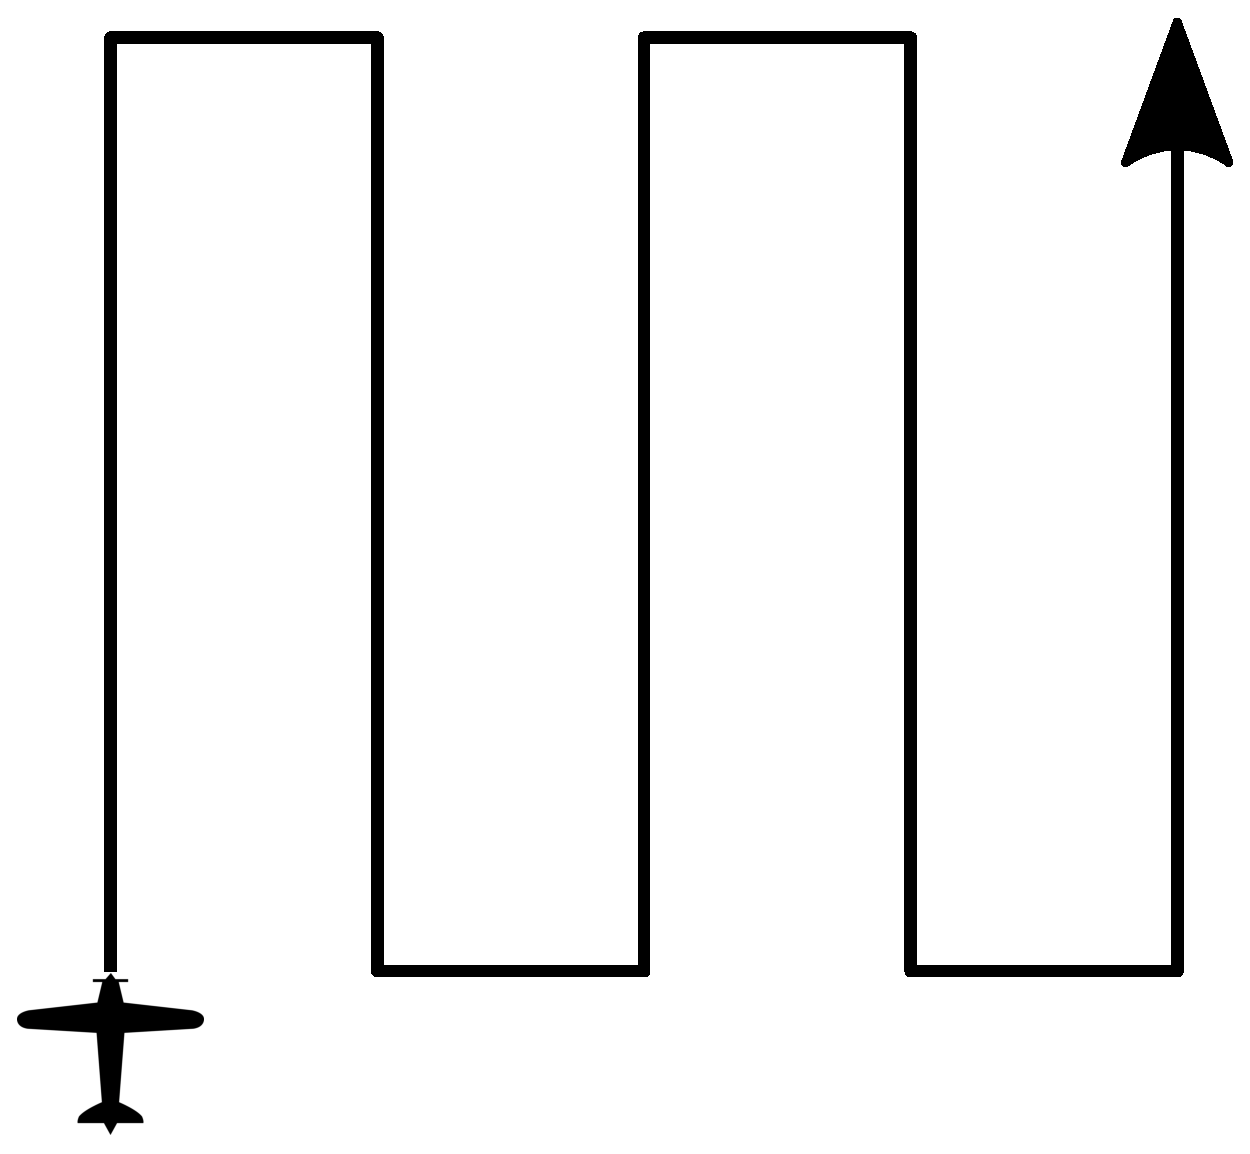
\includegraphics[width=1.0\textwidth]{SimpleLawnmower}
\caption[Simple Lawnmower]{This is the general form of a lawnmower pattern aerial imaging run} %TODO
\label{fig:simplelawnmower}
\end{figure}

